\documentclass[12pt,a4paper]{article}
\usepackage{amsmath,amssymb,mathrsfs,tikz,times,pifont}
\usepackage{enumitem}
\newcommand\circitem[1]{%
\tikz[baseline=(char.base)]{
\node[circle,draw=gray, fill=red!55,
minimum size=1.2em,inner sep=0] (char) {#1};}}
\newcommand\boxitem[1]{%
\tikz[baseline=(char.base)]{
\node[fill=cyan,
minimum size=1.2em,inner sep=0] (char) {#1};}}
\setlist[enumerate,1]{label=\protect\circitem{\arabic*}}
\setlist[enumerate,2]{label=\protect\boxitem{\alph*}}
%%%::::::by chnini ameur :::::::%%%
\everymath{\displaystyle}
\usepackage[left=1cm,right=1cm,top=1cm,bottom=1.7cm]{geometry}
\usepackage[colorlinks=true, linkcolor=blue, urlcolor=blue, citecolor=blue]{hyperref}
\usepackage{array,multirow}
\usepackage[most]{tcolorbox}
\usepackage{varwidth}
\usepackage{float} %pour utiliser l'option [H] qui force l'image à apparaître exactement à l'endroit où elle est placée dans le code.
\tcbuselibrary{skins,hooks}
\usetikzlibrary{patterns}
%%%::::::by chnini ameur :::::::%%%
\newtcolorbox{exa}[2][]{enhanced,breakable,before skip=2mm,after skip=5mm,
colback=yellow!20!white,colframe=black!20!blue,boxrule=0.5mm,
attach boxed title to top left ={xshift=0.6cm,yshift*=1mm-\tcboxedtitleheight},
fonttitle=\bfseries,
title={#2},#1,
% varwidth boxed title*=-3cm,
boxed title style={frame code={
\path[fill=tcbcolback!30!black]
([yshift=-1mm,xshift=-1mm]frame.north west)
arc[start angle=0,end angle=180,radius=1mm]
([yshift=-1mm,xshift=1mm]frame.north east)
arc[start angle=180,end angle=0,radius=1mm];
\path[left color=tcbcolback!60!black,right color = tcbcolback!60!black,
middle color = tcbcolback!80!black]
([xshift=-2mm]frame.north west) -- ([xshift=2mm]frame.north east)
[rounded corners=1mm]-- ([xshift=1mm,yshift=-1mm]frame.north east)
-- (frame.south east) -- (frame.south west)
-- ([xshift=-1mm,yshift=-1mm]frame.north west)
[sharp corners]-- cycle;
},interior engine=empty,
},interior style={top color=yellow!5}}
%%%%%%%%%%%%%%%%%%%%%%%

\usepackage{fancyhdr}
\usepackage{eso-pic}         % Pour ajouter des éléments en arrière-plan
% Commande pour ajouter du texte en arrière-plan
\usepackage{tkz-tab}
\AddToShipoutPicture{
    \AtTextCenter{%
        \makebox[0pt]{\rotatebox{80}{\textcolor[gray]{0.7}{\fontsize{5cm}{5cm}\selectfont PGB}}}
    }
}
\usepackage{lastpage}
\fancyhf{}
\pagestyle{fancy}
\renewcommand{\footrulewidth}{1pt}
\renewcommand{\headrulewidth}{0pt}
\renewcommand{\footruleskip}{10pt}
\fancyfoot[R]{
\color{blue}\ding{45}\ \textbf{2024}
}
\fancyfoot[L]{
\color{blue}\ding{45}\ \textbf{Prof:M. BA}
}
\cfoot{\bf
\thepage /
\pageref{LastPage}}

% Définition de l'encadré adaptatif avec fond jaune
\newtcolorbox{resultbox}{
    colback=red!30, % Fond rouge clair
    colframe=black, % Bordure noire fine
    sharp corners, % Coins nets
    boxrule=0.5pt, % Contour léger
    boxsep=2pt, % Espacement interne
    left=5pt, right=5pt, top=2pt, bottom=2pt, % Marges internes
}

\begin{document}
\renewcommand{\arraystretch}{1.5}
\renewcommand{\arrayrulewidth}{1.2pt}
\begin{tikzpicture}[overlay,remember picture]
\node[draw=blue,line width=1.2pt,fill=purple,text=blue,inner sep=3mm,rounded corners,pattern=dots]at ([yshift=-2.5cm]current page.north) {\begingroup\setlength{\fboxsep}{0pt}\colorbox{white}{\begin{tabular}{|*1{>{\centering \arraybackslash}p{0.28\textwidth}} |*2{>{\centering \arraybackslash}p{0.2\textwidth}|} *1{>{\centering \arraybackslash}p{0.19\textwidth}|} }
\hline
\multicolumn{3}{|c|}{$\diamond$$\diamond$$\diamond$\ \textbf{Lycée de Dindéfélo}\ $\diamond$$\diamond$$\diamond$ }& \textbf{A.S. : 2024/2025} \\ \hline
\textbf{Matière: Mathématiques}& \textbf{Niveau : T}\textbf{S2} &\textbf{Date: 09/12/2024} & \textbf{Durée : 4 heures} \\ \hline
\multicolumn{4}{|c|}{\parbox[c]{10cm}{\begin{center}
\textbf{{\Large\sffamily Correction du devoir n$ ^{\circ} $ 1 Du 1$ ^\text{\bf er} $ Semestre}}
\end{center}}} \\ \hline
\end{tabular}}\endgroup};
\end{tikzpicture}
\vspace{3cm}

\section*{\underline{Exercice 1 :} 0,5 $\times $ 10 = 5 points}

\begin{enumerate}

%--------------------- 1 -------------------------
\item \textbf{Théorème des valeurs intermédiaires (TVI).}  
Soit \(f\) une fonction continue sur l’intervalle \([a,b]\).  
Pour tout réel \(k\) compris entre \(f(a)\) et \(f(b)\), il existe \(c \in [a,b]\) tel que  
\[
f(c) = k.
\]

\textbf{Corollaire.}  
L’image d’un intervalle par une fonction continue est un intervalle.  
En particulier, si \(f(a)f(b) < 0\), alors \(f\) admet au moins une solution de l’équation \(f(x)=0\) dans \([a,b]\).

%--------------------- 2 -------------------------
\item \textbf{Théorème de la bijection.}  
Si \(f\) est continue et strictement monotone sur un intervalle \(I\), alors :
\begin{itemize}
    \item \(f\) est bijective de \(I\) vers \(J=f(I)\),
    \item l’application réciproque \(f^{-1} : J \to I\) est continue,
    \item \(f^{-1}\) est strictement monotone (même sens si \(f\) est croissante, sens opposé si \(f\) est décroissante).
\end{itemize}

%--------------------- 3 -------------------------
\item \textbf{Théorème des accroissements finis (TAF).}  
Si \(f\) est continue sur \([a,b]\) et dérivable sur \((a,b)\), alors il existe \(c \in (a,b)\) tel que :
\[
f'(c) = \frac{f(b) - f(a)}{b - a}.
\]

\textbf{Inégalité des accroissements finis (IAF).}  
Si de plus \(|f'(x)| \le M\) pour tout \(x \in (a,b)\), alors :
\[
|f(x) - f(y)| \le M |x - y|,\qquad \forall x,y \in [a,b].
\]

%--------------------- 4 -------------------------
\item \textbf{(Rappel) Théorème de la bijection.}  
Même énoncé que dans la question 2.

%--------------------- 5 -------------------------
\item \[
\text{Si } \lim_{x \to x_0} \frac{f(x)-f(x_0)}{x-x_0} = a \ (a \neq 0),
\]
alors \(f\) est dérivable en \(x_0\) et :
\[
f'(x_0) = a.
\]
En particulier, \(f\) est localement strictement monotone en \(x_0\) et \(x_0\) n’est pas un extremum.

%--------------------- 6 -------------------------
\item \[
\text{Si } \lim_{x \to x_0^-} \frac{f(x)-f(x_0)}{x-x_0} = +\infty,
\]
alors la dérivée à gauche de \(f\) en \(x_0\) est \(+\infty\).  
La pente est verticale du côté gauche (pas de dérivée finie).

%--------------------- 7 -------------------------
\item \[
\text{Si } \lim_{x \to x_0} \frac{f(x)-f(x_0)}{x-x_0} = 0,
\]
alors \(f\) est dérivable en \(x_0\) et :
\[
f'(x_0) = 0.
\]
La tangente en \(x_0\) est horizontale.

%--------------------- 8 -------------------------
\item Si
\[
\lim_{x \to +\infty} f(x) = +\infty, \qquad 
\lim_{x \to +\infty} \frac{f(x)}{x} = \beta \in \mathbb{R}^*, \qquad
\lim_{x \to +\infty} [f(x) - \beta x] = +\infty,
\]
alors la droite d’équation \(y = \beta x + b\) n’est \textbf{pas} une asymptote oblique pour \(f\).  
L'écart entre \(f(x)\) et \(\beta x\) diverge vers \(+\infty\).

%--------------------- 9 -------------------------
\item Si \(f\) est continue et strictement décroissante sur \(]-\infty, b]\), alors :
\[
f(]-\infty, b]) = (\ell,\, f(b)],
\]
où \(\displaystyle \ell = \lim_{x \to -\infty} f(x)\).
L’intervalle est ouvert à gauche car \(-\infty\) n’est pas un réel.
\end{enumerate}


\section*{\textcolor{green}{\underline{Exercice 2 :} 4 points}}

\begin{enumerate}
    \item Calculons les limites suivantes : \textbf{(3 × 1 pt)}
    \begin{align*}
    \lim_{x \to 0} \frac{\sqrt{1+\sin x} - 1}{\sin 2x}&=\lim_{x \to 0} \dfrac{\sin x }{\sin 2x\left( \sqrt{1+\sin x} + 1\right) }\\
    &=\lim_{x \to 0} \dfrac{\frac{\sin x}{x} }{\dfrac{2\sin 2x}{2x}}\times \dfrac{1}{\left(\sqrt{1+\sin x} + 1\right)}\\
    &=\dfrac{1}{2}\times\frac{1}{2}\\
    &=\dfrac{1}{4}
    \end{align*}
\[
\textcolor{green}{\boxed{ \lim_{x \to 0} \dfrac{\sqrt{1+\sin x} - 1}{\sin 2x}=\frac{1}{4}  }} \textbf{ 1 points}
\]

    \begin{align*}
    \lim_{x \to 0} \dfrac{\cos x - 1}{x^3 + x^2}&=\lim_{x \to 0}\dfrac{\cos x - 1}{x^2(x + 1)}\\
    &=\lim_{x \to 0} \dfrac{\cos x - 1}{x^{2}} \times \dfrac{1}{x+1}\\
    &=-\dfrac{1}{2}\times1\\
    &=-\dfrac{1}{2}
    \end{align*}
\[
\textcolor{green}{\boxed{ \lim_{x \to 0} \dfrac{\cos x - 1}{x^3 + x^2}=-\frac{1}{2}  }} \textbf{ 1 points}
\]

    \begin{align*}
    \lim_{x \to 1} \dfrac{\sqrt{x + 3} - \sqrt{5 - x}}{\sqrt{2x + 7} - \sqrt{10 - x}}&=\lim_{x \to 0}\dfrac{\left( \sqrt{x + 3} - \sqrt{5 - x}\right)\left( \sqrt{x + 3} + \sqrt{5 - x}\right)\left( \sqrt{2x + 7} - \sqrt{10 - x}\right) }{\left( \sqrt{2x + 7} - \sqrt{10 - x}\right) \left( \sqrt{2x + 7} - \sqrt{10 - x}\right) \left( \sqrt{x + 3} - \sqrt{5 - x}\right)}\\
    &=\lim_{x \to 1} \dfrac{\left[ x + 3 - (5 - x)\right]\left( \sqrt{2x + 7} + \sqrt{10 - x}\right) }{ \left[  2x + 7 - (10 - x) \right]  \left( \sqrt{x + 3} + \sqrt{5 - x}\right)}\\
    &=\lim_{x \to 1} \dfrac{2(-1+x)\left( \sqrt{2x + 7} + \sqrt{10 - x}\right) }{ 3( x - 1 )  \left( \sqrt{x + 3} + \sqrt{5 - x}\right)}\\
    &=\lim_{x \to 1} \dfrac{2(x-1)\left( \sqrt{2x + 7} + \sqrt{10 - x}\right) }{ 3( x - 1 )  \left( \sqrt{x + 3} + \sqrt{5 - x}\right)}\\
    &=\lim_{x \to 1} \dfrac{2\left( \sqrt{2x + 7} + \sqrt{10 - x}\right) }{ 3\left( \sqrt{x + 3} + \sqrt{5 - x}\right)}\\
    &=\dfrac{2}{3} \times \dfrac{6}{4}
    \end{align*}
\[
\textcolor{green}{\boxed{ \lim_{x \to 1} \dfrac{\sqrt{x + 3} - \sqrt{5 - x}}{\sqrt{2x + 7} - \sqrt{10 - x}}=1 }} \textbf{ 1 points}
\]

    \begin{align*}
    \lim_{x \to 1} \dfrac{\sin(\pi x)}{x - 1}&=\lim_{X \to 0}\dfrac{\sin(\pi X)}{X}\\
    																				&=\lim_{X \to 0}\pi\dfrac{\sin(\pi X)}{\pi X}\\
    																				&=1
    \end{align*}
\[
\textcolor{green}{\boxed{ \lim_{x \to 1} \dfrac{\sin(\pi x)}{x - 1}=1 }} \textbf{ 1 points}
\]

    \item Donnons les primitives des fonctions \(f\), \(g\) et \(h\) respectivement sur \(\mathbb{R}\) et \(\mathbb{R} \setminus \{1; 2\}\). \textbf{(2 × 0,5 pt)}

		\[ 
		f(x)=2\cos(x)-3\sin(x)
		\]    

		\[ F(x)=2\sin(x)+3\cos(x) + k \]    

    \[
     \textcolor{green}{\boxed{ F(x)=2\sin(x)+3\cos(x) + k }} \textbf{ 0,5 points}
    \]    
    
    \[
    g(x) = (3x-1)(3x^2-2x+3)^3 
    \]

		\[
    G(x) =\dfrac{1}{8}(3x^2-2x+3)^4+k
    \] 
       
    \[
     \textcolor{green}{\boxed{ G(x) =\dfrac{1}{8}(3x^2-2x+3)^4 + k }} \textbf{ 0,5 points}
    \]
    
    \[
    h(x) = \dfrac{1-x^2}{(x^3-3x+2)^3}.
    \]
    
    \[
     \textcolor{green}{\boxed{ H(x) = \dfrac{1}{3(x^3-3x+2)} + k }} \textbf{ 0,5 points}
    \]
\end{enumerate}

\section*{\underline{Problème :} 9,5 points}

\underline{\textbf{Partie A :}}
Soit la fonction $f$ définie par :
\[
f(x)=
\begin{cases}
\dfrac{x^2-2x}{x-1} & \text{si } x<0,\\[4mm]
x + \sqrt{x^2+x} & \text{si } x\ge 0,
\end{cases}
\qquad
\text{et } (\mathcal{C}_f) \text{ sa courbe représentative dans un repère orthonormé } (O,\vec{i},\vec{j}).
\]

\begin{enumerate}
    \item Déterminons l'ensemble de définition $\mathcal{D}_f$ de $f$. \hspace{1cm} \textbf{(0,5 pt)}

\(
\text{Posons }f(x)=
\begin{cases}
f_{1}(x) & \text{si } x<0,\\[4mm]
f_{2}(x) & \text{si } x\ge 0,
\end{cases}
\)    

\begin{itemize}
\item $ f_{1} \quad \exists \quad$ ssi  $x - 1x \neq 0 $ et $x<0$
		    
		    $x - 1 \neq 0 \implies x \neq 1$ et $x<0$

        \underline{$Df_{1} = ]-\infty ; 0[$}
\item $ f_{2} \quad \exists \quad$ ssi  $x^2 + x \geq 0 $ et $x\ge 0$

Posons $x^2 + x = 0 $

$x^2 + x = 0  \implies x=0 \textbf{ ou } x=-1$       
   
    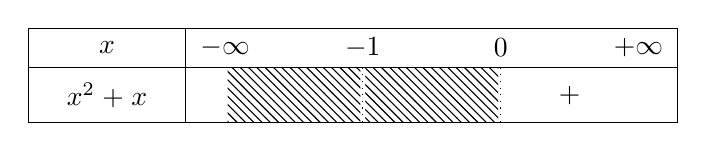
\begin{tikzpicture}[node style/.style={fill opacity=0,text opacity=1}]
        \tkzTabInit[espcl=1.75]{$x$/.5,$x^2 + x$/.7}{$-\infty$,$-1$,$0$,$+\infty$}
        \tkzTabLine{, h, t, h, t, +, }
    \end{tikzpicture}
    
    \underline{$Df_{2} = [0 ; +\infty[$}     
\end{itemize}

$$ \text{Donc}\quad
\begin{aligned}
Df & = Df_{1} \cup Df_{2} \\
    & = ]-\infty ; 0] \cup [0 ; +\infty[\\
    &=\mathbb{R} 
\end{aligned}
$$
    
    $$ \textcolor{red}{ \boxed{Df = \mathbb{R}} }$$
  
    \item Déterminons les limites aux bornes de $\mathcal{D}_f$. 

\begin{itemize}
\item \underline{En $-\infty$}: $f(x)=f_{1}(x)$   
    
\(
\begin{aligned}
 \lim\limits_{x \to -\infty} f(x) &= \lim\limits_{x \to -\infty} \dfrac{x^2-2x}{x-1}\\
 																	&= \lim\limits_{x \to -\infty} \dfrac{x^2}{x}\\
 																	&= \lim\limits_{x \to -\infty} x\\
 																	&= -\infty
\end{aligned}    
\)

\textcolor{red}{{\underline{$\lim\limits_{x \to -\infty} f(x) = -\infty$}}} \hspace{1cm} \textbf{(0,25 pt)}

\item \underline{En $+\infty$}: $f(x)=f_{2}(x)$   
    
\(
\begin{aligned}
 \lim\limits_{x \to +\infty} f(x) &= \lim\limits_{x \to +\infty} x + \sqrt{x^2+x}\\
 																	&= \lim\limits_{x \to +\infty} x + \sqrt{x^2+x}\\
 																	&= \lim\limits_{x \to +\infty} \\
 																	&= 
\end{aligned}    
\)

\textcolor{red}{{\underline{$\lim\limits_{x \to +\infty} f(x) = +\infty$}}} \hspace{1cm} \textbf{(0,25 pt)}
\end{itemize}

    \item Étudions la continuité et la dérivabilité de $f$ en $0$. Interprétons les résultats obtenus. \hspace{1cm} \textbf{(1,5 pt)}

\underline{\textbf{Etudions la Continuité de f en 0  } } 

 \begin{itemize}
\item \underline{En $0^-$}: $f(x)=f_{1}(x)$   
    
\(
\begin{aligned}
 \lim\limits_{x \to 0^-} f(x) &= \lim\limits_{x \to 0^-} \dfrac{x^2-2x}{x-1}\\
 															&= 0
\end{aligned}    
\)

\textcolor{red}{{\underline{$\lim\limits_{x \to 0^-} f(x) = 0$}}}

\item \underline{En $0^+$}: $f(x)=f_{2}(x)$   
    
\(
\begin{aligned}
 \lim\limits_{x \to 0^+} f(x) &= \lim\limits_{x \to 0^+} x + \sqrt{x^2+x}\\
															&=0
\end{aligned}    
\)

\textcolor{red}{{\underline{$\lim\limits_{x \to 0^+} f(x) = 0$}}}
\end{itemize}   

On a $f(0)=0$

\textcolor{red}{Finalement $\lim\limits_{x \to 0^-} f(x) = \lim\limits_{x \to 0^+} f(x) = f(0)$ donc f est continue en $0$}

\underline{\textbf{Etudions la dérivabilité de f en 0  } } 

\begin{itemize}
\item \underline{En $0^-$}: $f(x)=f_{1}(x)$ 

\(
\begin{aligned}
 \lim\limits_{x \to 0^-} \dfrac{f(x)-f(0)}{x} &= \lim\limits_{x \to 0^-} \dfrac{\dfrac{x^2-2x}{x-1}}{x}\\
 															                &= \lim\limits_{x \to 0^-} \dfrac{x^2-2x}{x^2-x}\\
 															                &= \lim\limits_{x \to 0^-} \dfrac{x-2}{x-1}\\
 															                &=2
\end{aligned}    
\)

\textcolor{red}{ $f$ est dérivable à gauche de $0$ et $y=2x$ est une démi-tangent en $0^-$ }

\item \underline{En $0^+$}: $f(x)=f_{2}(x)$ 

\(
\begin{aligned}
\lim\limits_{x \to 0^+} \dfrac{f(x)-f(0)}{x} &=\lim\limits_{x \to 0^+} \dfrac{x + \sqrt{x^2+x}}{x}\\
															               &=\lim\limits_{x \to 0^+} \dfrac{x^2-x^2-x}{x(x - \sqrt{x^2+x})}\\
															               &=\lim\limits_{x \to 0^+} \dfrac{-x}{x(x - \sqrt{x^2+x})}\\
															               &=\lim\limits_{x \to 0^+} \dfrac{-1}{(x - \sqrt{x^2+x})}\\
															               &="\dfrac{-1}{0}"\\
\end{aligned}    
\)

Supposons que $ x - \sqrt{x^2+x} > 0 $

$ x - \sqrt{x^2+x} > 0 \implies \sqrt{x^2+x} < x $

$
\begin{aligned}
\sqrt{x^2+x} < x &\implies \begin{cases}
										x^2+x > 0\\
										x > 0\\ 
										x^2+x < x^{2} 
										\end{cases}\\
									&\implies \begin{cases}
										x^2+x > 0\\
										x > 0\\ 
										x < 0
										\end{cases}\\
\end{aligned}
$

$
\begin{aligned}
\begin{cases}
x^2+x = 0\\
x = 0 
\end{cases}\implies
\begin{cases}
x=0 \textbf{ ou } x=-1\\
x = 0
\end{cases}
\end{aligned}
$

    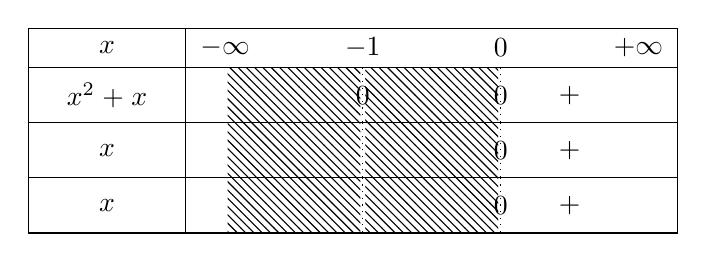
\begin{tikzpicture}[node style/.style={fill opacity=0,text opacity=1}]
        \tkzTabInit[espcl=1.75]{$x$/.5,$x^2 + x$/.7,$x$/.7,$x$/.7}{$-\infty$,$-1$,$0$,$+\infty$}
        \tkzTabLine{,h,z,h,z,+, }
        \tkzTabLine{,h,t,h,z,+, }
        \tkzTabLine{,h,t,h,z,+, }
    \end{tikzpicture}

$$ S = \emptyset $$ Ainsi, il n'existe pas de $ x > 0 $ pour lequel $ x-\sqrt{x^2+x} > 0  $

 $$ \textbf{Donc } x-\sqrt{x^2+x} <0,  \, \forall x\in ]0;+\infty[ $$

\textcolor{red}{Ainsi  $\forall x\in ]0;+\infty[$ $f'(x) > 0 $ donc f  est croissant $0;+\infty[$}

\(
\begin{aligned}
\lim\limits_{x \to 0^+} \dfrac{f(x)-f(0)}{x} &=\lim\limits_{x \to 0^+} \dfrac{-1}{(x - \sqrt{x^2+x})}\\
															               &=\dfrac{-1}{0^-}\\
															               &=+\infty \\
\end{aligned}    
\)

\textcolor{red}{ $f$ n'est pas dérivable à droite de $0$ donc admet une démi-tangent orientée vers le haut en $0^+$  }

\end{itemize}     
    
    \item 
      \begin{enumerate}
        \item Montrons que $(\mathcal{C}_f)$ admet en $-\infty$ une asymptote oblique $\Delta_1$ dont on déterminera l’équation. \textbf{(0,5 pt)}

Comme $\lim\limits_{x \to -\infty} f(x) = -\infty$  

\begin{itemize}
\item Cherchons  $\lim\limits_{x \to -\infty} \dfrac{f(x)}{x} $  

\(
\begin{aligned}
 \lim\limits_{x \to -\infty} \dfrac{f(x)}{x} &= \lim\limits_{x \to -\infty} \dfrac{\dfrac{x^2-2x}{x-1}}{x}\\
 																	&= \lim\limits_{x \to -\infty} \dfrac{x^2-2x}{x^2-x}\\
 																	&= \lim\limits_{x \to -\infty} \dfrac{x^2}{x^2}\\
 																	&= 1
\end{aligned}    
\)        

Donc  $\lim\limits_{x \to -\infty} \dfrac{f(x)}{x} = 1 $       

\item Cherchons  $\lim\limits_{x \to -\infty} f(x)-x $ 

\(
\begin{aligned}
 \lim\limits_{x \to -\infty} f(x)-x &= \lim\limits_{x \to -\infty} \dfrac{x^2-2x}{x-1}-x\\
 																	&= \lim\limits_{x \to -\infty} \dfrac{x^2-2x-x^2+x}{x-1}\\
 																	&= \lim\limits_{x \to -\infty} \dfrac{-x}{x-1}\\
 																	&= \lim\limits_{x \to -\infty} \dfrac{-x}{x}\\
 																	&= -1
\end{aligned}    
\) 

\textcolor{red}{Donc $(\Delta_1)$: $ y = x - 1$ est une asymptote oblique à $(\mathcal{C}_f)$ en $-\infty$ } 
  
\end{itemize}      
        
        \item Étudions la position relative de $(\mathcal{C}_f)$ par rapport à $\Delta_1$ sur $]-\infty;0[$. \hspace{1cm} \textbf{(0,5 pt)}
        
        Etudions le signe de $f(x)-y$ 

\(
\begin{aligned}
f(x)-y &= f(x)-(x-1)\\
 			 &= \dfrac{x^2-2x}{x-1}-(x-1)\\
 			 &= x-1-\dfrac{1}{x-1}-x+1\\
 			 &= -\dfrac{1}{x-1}\\
\end{aligned}    
\)      
    
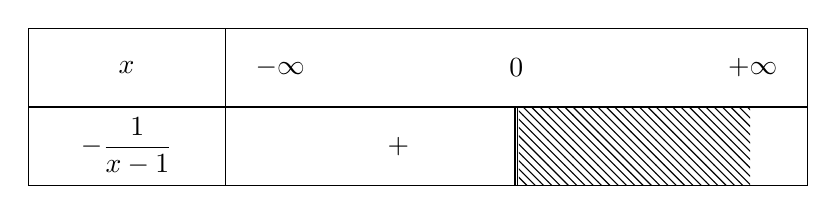
\begin{tikzpicture}
   \tkzTabInit[lgt = 2.5, espcl = 3, deltacl = 0.7]{$x$ / 1 , $-\dfrac{1}{x-1}$ / 1 }{$-\infty$, $0$, $+\infty$}
   \tkzTabLine{,+,d,h,}
\end{tikzpicture}
        
Sur $]-\infty;0[,\, f(x)-y > 0 $ donc $(\mathcal{C}_f)$ est au-dessus de $(\Delta_1)$


      \end{enumerate}
    \item Montrons que $(\mathcal{C}_f)$ admet en $-\infty$ une asymptote oblique $(\Delta_1)$ dont on déterminera l’équation. \textbf{(0,5 pt)}

Comme $\lim\limits_{x \to +\infty} f(x) = +\infty$  

\begin{itemize}
\item Cherchons  $\lim\limits_{x \to -\infty} \dfrac{f(x)}{x} $  

\(
\begin{aligned}
 \lim\limits_{x \to +\infty} \dfrac{f(x)}{x} &= \lim\limits_{x \to +\infty}  \dfrac{x + \sqrt{x^2+x}}{x}\\
 																	&= \lim\limits_{x \to +\infty} \dfrac{x\left(1 + \sqrt{1+\dfrac{1}{x}}\right)}{x}\\
 																	&= \lim\limits_{x \to +\infty} \left(1 + \sqrt{1+\dfrac{1}{x}}\right)\\
 																	&= 2
\end{aligned}    
\)        

Donc  $\lim\limits_{x \to +\infty} \dfrac{f(x)}{x} = 2 $       

\item Cherchons  $\lim\limits_{x \to +\infty} f(x)-2x $ 

\(
\begin{aligned}
 \lim\limits_{x \to +\infty} f(x)-2x &= \lim\limits_{x \to +\infty} x + \sqrt{x^2+x}-2x\\
 																		 &= \lim\limits_{x \to +\infty} \sqrt{x^2+x}-x\\
 																		 &= \lim\limits_{x \to +\infty} \dfrac{x^2+x-x^2}{\sqrt{x^2+x}+x} \\
 																		 &= \lim\limits_{x \to +\infty} \dfrac{x}{\sqrt{x^2+x}+x} \\
 																		 &= \lim\limits_{x \to +\infty} \dfrac{x}{x\left(1 + \sqrt{1+\dfrac{1}{x}}\right)} \\
 																		 &= \lim\limits_{x \to +\infty} \dfrac{1}{\left(1 + \sqrt{1+\dfrac{1}{x}}\right)} \\
 																	   &= \dfrac{1}{2}
\end{aligned}    
\)   
 
\end{itemize}
  		    
    \textcolor{red}{Donc $(\Delta_2)$: $ y = 2x+\dfrac{1}{2}$ est une asymptote oblique à $(\mathcal{C}_f)$ en $+\infty$ }
    
    \item Précisons l'ensemble de dérivabilité de $f$ puis calculons $f'(x)$ sur chaque intervalle où $f$ est dérivable.\\ \textbf{(0,5 pt)}   

\[ Df' = \mathbb{R}^*\]    

\[
f(x)=
\begin{cases}
\dfrac{x^2-2x}{x-1} & \text{si } x<0,\\[4mm]
x + \sqrt{x^2+x} & \text{si } x\ge 0,
\end{cases}
\qquad
\text{et } (\mathcal{C}_f) \text{ sa courbe représentative dans un repère orthonormé } (O,\vec{i},\vec{j}).
\]

\[
\begin{aligned}
f'(x)=
\begin{cases}
\dfrac{(2x-2)(x-1)-(x^2-2x)}{(x-1)^{2}} & \text{si } x<0,\\[4mm]
1 + \dfrac{2x+1}{2\sqrt{x^2+x}} & \text{si } x > 0,
\end{cases}&\implies
\begin{cases}
\dfrac{2x^2-2x-2x+2-x^2+2x}{(x-1)^{2}} & \text{si } x<0,\\[4mm]
\dfrac{2\sqrt{x^2+x}+2x+1}{2\sqrt{x^2+x}} & \text{si } x > 0,
\end{cases}\\
&\implies
\begin{cases}
\dfrac{x^2-2x+2}{(x-1)^{2}} & \text{si } x<0,\\[4mm]
\dfrac{2\sqrt{x^2+x}+2x+1}{2\sqrt{x^2+x}} & \text{si } x > 0,
\end{cases}
\end{aligned}
\]    
    
    \item Dressons le tableau de variation de $f$. \hspace{1cm} \textbf{(0,5 pt)}

\begin{itemize}
\item Si \( x<0\,, f(x)=\dfrac{x^2-2x+2}{(x-1)^{2}} \)  le signe dépend du numérateur 

\( x^2-2x+2 = 0 \implies \Delta <0 \)
\textcolor{red}{ Ansi, si \( x<0\,, f(x) > 0 \)  donc f est croissante sur $]-\infty; 0[$}
\item Si $ x>0\,, f(x)= \dfrac{2\sqrt{x^2+x}+2x+1}{2\sqrt{x^2+x}}$ le signe dépend du numérateur 

%Supposons que $ 2\sqrt{x^2+x}+2x+1 < 0 $

%$ 2\sqrt{x^2+x}+2x+1 < 0 \implies \sqrt{x^2+x} < -\dfrac{2x+1}{2}$

%$
%\begin{aligned}
%\sqrt{x^2+x} < -\dfrac{2x+1}{2} &\implies \begin{cases}
																						%x^2+x > 0\\
																						%-\dfrac{2x+1}{2} > 0\\ 
																						%x^2+x < \left( -\dfrac{2x+1}{2} \right)^{2} 
																						%\end{cases}\\
											 %&\implies \begin{cases}
																						%x^2+x > 0\\
																						%2x+1 < 0\\ 
																						%x^2+x < x^{2}+x+\dfrac14 
																						%\end{cases}\\
											%&\implies \begin{cases}
																						%x^2+x > 0\\
																						%2x+1 < 0\\ 
																						%0 < \dfrac14 
																						%\end{cases}\\
%\end{aligned}
%$

%$
%\begin{aligned}
%\begin{cases}
%x^2+x = 0\\
%2x+1 = 0 
%\end{cases}\implies
%\begin{cases}
%x=0 \textbf{ ou } x=-1\\
%x = -\dfrac{1}{2}
%\end{cases}
%\end{aligned}
%$

    %\begin{tikzpicture}[node style/.style={fill opacity=0,text opacity=1}]
     %   \tkzTabInit[espcl=1.75]{$x$/.5,$x^2 + x$/.7,$2x + 1$/.7}{$-\infty$,$-1$,$-\dfrac{1}{2}$,$0$,$+\infty$}
     %   \tkzTabLine{,h,z,h,t,h,z,+, }
     %   \tkzTabLine{,h,t,h,z,h,t,+, }
    %\end{tikzpicture}

%$$ S = \emptyset $$ Ainsi, il n'existe pas de $ x > 0 $ pour lequel $ 2\sqrt{x^2+x}+2x+1 < 0  $

% $$ \textbf{Donc } 2\sqrt{x^2+x}+2x+1 > 0 \, \forall x\in ]0;+\infty[ $$

%\textcolor{red}{Ainsi  $\forall x\in ]0;+\infty[$ $f'(x) > 0 $ donc f  est croissant $0;+\infty[$}
  
$$ \textbf{Or } 2\sqrt{x^2+x}+2x+1 > 0 \, \forall x\in ]0;+\infty[ $$

\textcolor{red}{Ainsi  $\forall x\in ]0;+\infty[$ $f'(x) > 0 $ donc f  est croissant $0;+\infty[$}
\end{itemize}
    
    
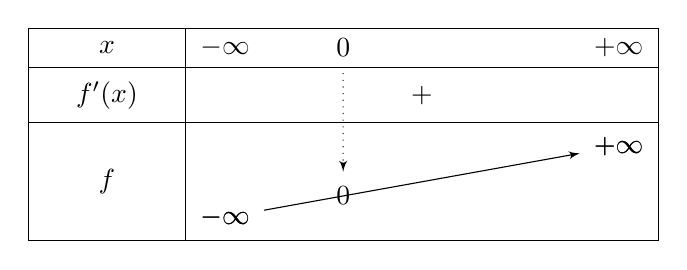
\begin{tikzpicture}[node style/.style={fill opacity=0,text opacity=1}]
        \tkzTabInit[espcl=5]{$x$/.5,$f'(x)$/.7,$f$/1.5}{$-\infty$,$+\infty$}
        \tkzTabLine{,+,}
        \tkzTabVar{-/$-\infty$,+/$+\infty$/}
        \tkzTabVal[draw]{1}{2}{0.3}{$0$}{$0$}
\end{tikzpicture}   
  
++++++++++++++++++++++++

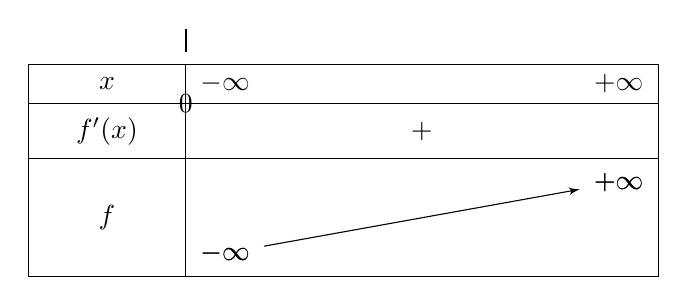
\begin{tikzpicture}[node style/.style={fill opacity=0,text opacity=1}]
    \tkzTabInit[espcl=5]{$x$/.5,$f'(x)$/.7,$f$/1.5}{$-\infty$,$+\infty$}

    \tkzTabLine{,+,}

    \tkzTabVar{-/$-\infty$,+/$+\infty$/}

    % Trace deux petits traits pour non dérivabilité en 0
    \node at (2,0.3) {}; % position du point
    \draw[thick] (2,0.15) -- (2,0.45);
    \draw[thick] (2,0.25) -- (2,0.35);
    
    % Optionnel : écrire f(0)=0
    \node at (2,-0.5) {$0$};
\end{tikzpicture}



+++++++++++++++++++++++++

    \item Précisons les points d'intersection de $(\mathcal{C}_f)$ avec les axes du repère. \textbf{(0,25 pt)}

\begin{itemize}
\item Pour $ x<0 $, $ f(x)= \dfrac{x^2-2x}{x-1} $

\begin{itemize}
\item Avec $(ox)$, nous ne pouvons pas calculer $f(0)$ car $ x<0 $

\item Avec $(oy)$ résolvons $f(x)=0$

$ 
\begin{aligned}
f(x)=0 &\implies \dfrac{x^2-2x}{x-1} = 0\\
			&\implies x= 0 \text{ ou } x=2 \text{ Or } x<0\\
\end{aligned}
$

\end{itemize}

\item Pour $ x \geq 0 $, $ f(x)= x + \sqrt{x^2+x}$
\begin{itemize}
\item Avec $(ox)$, $ f(0)= 0$

\item Avec $(oy)$ résolvons $f(x)=0$
\(
\implies x+\sqrt{x^2+x}=0.
\)

\(
\sqrt{x^2+x}=-x,
\)

En élevant au carré : \(x^2+x=x^2\Rightarrow x=0\).

Donc la solution est 0


\end{itemize}

\end{itemize}
 
    \item Construire la courbe $(\mathcal{C}_f)$. \hspace{1cm} \textbf{(1,5 pt)}    

\begin{center}
\begin{figure}[H]% Forcer l'image à cet endroit
\centering
\includegraphics[width=0.8\textwidth]{devoir1-2025-2026.png}
\caption{Courbe de (Cf)}
\label{fig:monimage}
\end{figure}
\href{https://www.geogebra.org/classic/wkappehb}{Clique ici pour voir la courbe sur géogébra}
\end{center}

\end{enumerate}

\underline{\textbf{Partie B :}}

Soit $h$ la restriction de $f$ à l’intervalle $I = [0; +\infty[$.

\begin{enumerate}

    \item Montrons que $h$ réalise une bijection de $I$ dans un intervalle $J$ que l'on  précisera.
    \hspace{1cm} \textbf{(0,25 pt)}
    
    Sur $I$ $h$ est continue est strictement croissante donc réalise une bijection de $I$ vers $J=[0,+\infty[$

    \item La bijection réciproque $h^{-1}$ est-elle dérivable sur $J$ ?
    \hspace{1cm} \textbf{(0,25 pt)}

		Comme $\forall x \in I$, $h'(x)\neq 0$ donc $h^{-1}$ est dérivable sur $J$

    \item Calculons $h\!\left(\dfrac{4}{5}\right)$ puis $(h^{-1})'(2)$.
   \hspace{1cm} \textbf{(0,5 pt)}

\(
\begin{aligned}
h\!\left(\frac{4}{5}\right)
&= \frac{4}{5} + \sqrt{\left(\frac{4}{5}\right)^2 + \frac{4}{5}}\\
&= \frac{4}{5} + \sqrt{\frac{16}{25} + \frac{20}{25}}\\
&= \frac{4}{5} + \frac{6}{5}\\
&= \frac{10}{5}\\
&= 2
\end{aligned}
\)

\begin{resultbox}
    \[
        \mathbf{h\!\left(\frac{4}{5}\right)=2}
    \]
\end{resultbox}

On a : $(h^{-1})'(2) = \dfrac{1}{h'\left(\frac{4}{5}\right)}$ et $h'(x)=\dfrac{1}{\dfrac{2\sqrt{x^2+x}+2x+1}{2\sqrt{x^2+x}}}$

$h'(2)=\dfrac{1}{\dfrac{2\sqrt{\left(\frac{4}{5}\right)^2+\left(\frac{4}{5}\right)}+2\left(\frac{4}{5}\right)+1}{2\sqrt{\left(\frac{4}{5}\right)^2+\left(\frac{4}{5}\right)}}}$

\(
\begin{aligned}
(h^{-1})'(2)
&= \dfrac{1}{h'\!\left(\frac{4}{5}\right)}\\[0.2cm]
&=\dfrac{1}{\dfrac{2\sqrt{\left(\frac{4}{5}\right)^2+\left(\frac{4}{5}\right)}+2\left(\frac{4}{5}\right)+1}{2\sqrt{\left(\frac{4}{5}\right)^2+\left(\frac{4}{5}\right)}}}\\[0.2cm]
&=\dfrac{2\sqrt{\left(\frac{4}{5}\right)^2+\left(\frac{4}{5}\right)}}
       {2\sqrt{\left(\frac{4}{5}\right)^2+\left(\frac{4}{5}\right)}+2\left(\frac{4}{5}\right)+1}\\[0.2cm]
&=\dfrac{2\cdot \frac{6}{5}}{2\cdot \frac{6}{5} + \frac{8}{5} + 1}\\[0.2cm]
&=\dfrac{\frac{12}{5}}{\frac{12}{5}+\frac{8}{5}+\frac{5}{5}}\\[0.2cm]
&=\dfrac{\frac{12}{5}}{\frac{25}{5}}\\[0.2cm]
&=\dfrac{12}{25}
\end{aligned}
\)


\begin{resultbox}
    \[
        \mathbf{(h^{-1})'(2)=\frac{12}{25}}
    \]
\end{resultbox}

    \item Construction de  $(\mathcal{C}_{h^{-1}})$ la courbe représentative de $h^{-1}$ dans le même repère.
    \hspace{1cm} \textbf{(0,5 pt)}
\begin{center}
\begin{figure}[H]% Forcer l'image à cet endroit
\centering
\includegraphics[width=0.8\textwidth]{devoir12025-2026Courbe2.png}
\caption{Courbe de (Cf)}
\label{fig:monimage}
\end{figure}
\href{https://www.geogebra.org/classic/wkappehb}{Clique ici pour voir la courbe sur géogébra}
\end{center}
    \item Exprimons $h^{-1}(x)$ pour tout $x \in J$.
    \hspace{1cm} \textbf{(0,5 pt)}

\[
\text{Soit } y = h(x) = x+\sqrt{x^{2}+x}.
\]

On isole la racine :
\[
y-x = \sqrt{x^{2}+x}.
\]

En élevant au carré, on obtient :
\[
(y-x)^{2} = x^{2}+x.
\]

\[
y^{2}-2xy+x^{2} = x^{2}+x.
\]

En simplifiant :
\[
y^{2}-2xy = x.
\]

On factorise par \(x\) :
\[
y^{2} = x(1+2y).
\]

D’où :

\begin{resultbox}
    \[
        \mathbf{h^{-1}(x)=\dfrac{x^{2}}{1+2x}}
    \]
\end{resultbox}


\end{enumerate}

\end{document}
